\chapter{Abelian Groups}
\label{ch:abelian}

\section{Brief overview of the chapter}

\section{Abelian groups}
\label{sec:abelian-groups}

%% Remove/modify once the rest of the section is being refactored with
%% new notation/style for identity types.
Recall that given a pointed type $X$, we coerce it silently to its
underlying unpointed type $X_\div$ whenever this coercion can be
inferred from context. For example, given a group $G$, the type
$\BG\weq \BG$ can not possibly mean anything but
$\BG_\div\simeq \BG_\div$ as the operator ``$\weq$'' acts on bare
types. To refer to the type of pointed equivalences (that is the
pointed functions whose underlying functions are equivalences), we
shall use the notation $\BG \ptdweto \BG$.%

\subsection{Center of a group}
\label{sec:center-group}

\begin{definition}
  Let $G$ be a group. The {\em center} of $G$, denoted
  $\grpcenter(G)$, is the group
  $\Aut_{(\BG_\div\eqto\BG_\div)}(\refl{\BG_\div})$.%
  \marginnote{%
    We work transparently through the equivalence
    \begin{displaymath}
      (\BG_\div=\BG_\div) \weq (\BG \weq \BG)
    \end{displaymath}
    so that $\id_{\BG_\div}$ is freely used in place of
    $\refl {\BG_\div}$ when convenient.%
  }%
\end{definition}

There is a natural map
$\ev_{\shape_G} : (\BG_\div\eqto\BG_\div) \to \BG_\div$ defined by
$\ev_{\shape_G}(\varphi)\defequi \varphi(\shape_G)$, where the path
$\varphi$ is coerced to a function through univalence. In particular,
$\ev_{\shape_G}(\refl{\BG_\div}) \jdeq \shape_G$. It makes the
restriction of this map to the connected component of
$\refl{\BG_\div}$ a pointed map. In other words, it defines a group
homomorphism
\begin{displaymath}
  \grpcenterinc G : \Hom(\grpcenter(G), G).
\end{displaymath}
such that $\B \grpcenterinc G \defequi \ev_{\shape_G}$. We will now
justify the name {\em center} for $\grpcenter(G)$, and connect it to
the notion of center for abstract groups in ordinary mathematics. The
homomorphism $\grpcenterinc G$ induces a homomorphism of abstract
groups from $\abstr(\grpcenter(G))$ to $\abstr(G)$. By induction on
$p:\refl{\BG_\div} \eqto \varphi$ for
$\varphi:\BG_\div \eqto \BG_\div$, one proves that
$\ap{\B \grpcenterinc G}(p) = p(\shape_G)$: indeed, this is true when
$p\jdeq \refl {\refl{\BG_\div}}$. One proves furthermore, again by
induction on $p:\refl{\BG_\div} \eqto \varphi$, that
$\ap \varphi = (q\mapsto \inv{p(\shape_G)} q p(\shape_G))$. In
particular, when $\varphi \jdeq \refl{\BG_\div}$, it shows that for
every $p:\refl{\BG_\div}\eqto\refl{\BG_\div}$, the following proposition
holds:
\begin{displaymath}
  \prod_{g:\USymG }p(\shape_G) g = g p(\shape_G)
\end{displaymath}
In other words, $\abstr{(\grpcenterinc G)}$ maps elements of
$\abstr(Z(G))$ to elements of $\abstr(G)$ that commute with every
other elements. (The set of these elements is usually called the
center of the group $\abstr(G)$ in ordinary group theory.)

\begin{lemma}
  \label{lemma:center-is-subgroup}%
  The map $\B \grpcenterinc G$ is a \covering over $\BG$.
\end{lemma}
\begin{proof}
  One wants to prove the proposition
  $\isset(\inv{(\B\grpcenterinc G)}(x))$ for each $x:\BG$. By
  connectedness of $\BG$, it reduces to showing the proposition only
  at $x\jdeq \shape_G$. However,
  \begin{displaymath}
    \inv{(\B\grpcenterinc G)}(\shape_G) \defequi \sum_{\varphi:{\B\grpcenter(G)}}{\shape_G \eqto \varphi(\shape_G)}
  \end{displaymath}
  Recall that $\B\grpcenter(G)$ is the connected component of
  $\refl{\BG_\div}$ in $\BG_\div \eqto \BG_\div$. In particular, if
  $(\varphi,p)$ and $(\psi,q)$ are two elements of the type on the
  right hand-side above, %  their identity type
  % $(\varphi,p)\eqto(\psi,q)$ is equivalent to their identity type in
  % $\BG_\div \eqto \BG_\div$, or in other words
  the characterization of identity types in sum types gives an
  equivalence:
  \begin{displaymath}
    ((\varphi,p) \eqto (\psi,q)) \equivto \sum_{\pi:\varphi\eqto\psi}\pi(\shape_G) p = q.
  \end{displaymath}
  We shall prove that the type on the right is a proposition, and it goes as
  follows:
  \begin{enumerate}
  \item for $\pi:\varphi\eqto\psi$, the type $\pi(\shape_G) p = q$ is a
    proposition; hence $\sum_{\pi:\varphi\eqto\psi}\pi(\shape_G) p = q$ is a
    subset of the set $\varphi \eqto \psi$, so for elements $(\pi,!)$ and
    $(\pi',!)$ of the subset, we have to prove $\pi=\pi'$,
  % \item for all $x:\BG$, $\varphi(x)=\psi(x)$ is a set, hence for
  %   $\pi,\pi':\varphi=\psi$, the type $\pi=\pi'$ is a proposition,
  \item because $\pi=\pi'$ is a proposition, by connectedness of $\BG$, it is
    enough to prove $\pi(\shape_G)=\pi'(\shape_G)$,
  \item finally the propositional condition on $\pi$ and $\pi'$ allows us to
    conclude that $\pi(\shape_G)= q\inv p = \pi'(\shape_G)$.
  \end{enumerate}
\end{proof}

\begin{corollary}
  \label{lemma:center-inc-inj-on-paths}%
  The induced map
  $\abstr {(\grpcenterinc G)}: \abstr(\grpcenter(G)) \to \abstr(G)$ is
  injective.
\end{corollary}

The following result explains how every element of the ``abstract
center'' of $G$ is picked out by $\abstr{(\grpcenterinc G)}$.
\begin{lemma}
  \label{lemma:center-inc-surj-on-paths}%
  Let $g:\USymG$ and suppose that $gh=hg$ for every
  $h:\USymG$. The fiber $\inv{(\ap {\B\grpcenterinc G})}(g)$ contains
  an element.
\end{lemma}
\begin{proof}
  One must construct an element $\hat g:\refl{\BG_\div} = \refl{\BG_\div}$ such
  that $g=\hat g(\shape_G)$. We shall use function extensionality and produce an
  element $\hat g(x):x\eqto x$ for all $x:\BG$ instead. Note that $x\eqto x$ is
  a set, and that connectedness of $\BG$ is not directly applicable here. We
  will use a technique that has already proven useful in many situations in the
  book, along the lines of the following sketch:
  \begin{enumerate}
  \item for a given $x:\BG$, if such a $\hat g(x):x\eqto x$ existed, it would
    produce an element of the type $T(\hat g(x))$ for a carefully chosen type
    family $T$,
  \item aim to prove $\iscontr(\sum_{u:x\eqto x}T(u))$ for any $x:\BG$,
  \item this is a proposition, so connectedness of $\BG$ can be applied
    and only $\iscontr(\sum_{u:\USymG}T(u))$ needs to be proven,
  \item hopefully, $\sum_{u:\USymG}T(u)$ reduces to an obvious
    singleton type.
  \end{enumerate}
  Here, for any $x:\BG$, we define the type family $T: (x\eqto x) \to \UU$
  by
  \begin{displaymath}
    T(q) \defequi \prod_{p:\shape_G\eqto x} (pg=qp).
  \end{displaymath}
  And we claim that $\sum_{q:x\eqto x}T(q)$ is contractible for any
  $x:\BG$. Because this is a proposition, one only need to check that it holds
  on one point of the connected type $\BG$, say $x\jdeq \shape_G$. We consider
  the following composition of equivalences:
  \begin{displaymath}%
    \begin{aligned}
      \sum_{q:\USymG}T(q) &\jdeq
      \sum_{q:\USymG}\prod_{p:\USymG}(pg=qp)
      \\
      &\equivto \sum_{q:\USymG}\prod_{p:\USymG}(g=q)
      \\
      &\equivto \sum_{q:\USymG}\USymG\to (g=q)
      \\
      &\equivto \sum_{q:\USymG}\Trunc{\USymG}\to (g=q)
      \\
      &\equivto \sum_{q:\USymG} (g=q)
      \\
      &\equivto 1
    \end{aligned}
  \end{displaymath}%
  % \marginnote[-10\baselineskip]{%
  In that composition, the first equivalence is using that $g$ commutes with
  every other element $p:\USymG$, so that $pg \inv p = g$. The second
  equivalence acknowledges the fact that the codomain $(g=q)$ does not depend on
  $p$ anymore, so that the dependent function type inside the sum is a simple
  function type. The third equivalence uses the universal property of
  propositional truncation under the sum. The fourth equivalence is the
  evaluation at $\trunc{\refl {\shape_G}}$ under the sum. The last equivalence
  is the contractibility of singleton types.%
  % }%

  We have just shown that for all $x:\BG$, the type $\sum_{q:x\eqto x}T(q)$ is
  contractible. We define now $\hat g(x):x\eqto x$ as the chosen center of
  contraction of that type. More precisely, by connectedness of $\BG$, the
  inverse $\inv\varphi$ of the exhibited equivalence
  $\varphi:\sum_{q:\USymG}T(q) \equivto 1$ produces a dependent function of
  type $\prod_{x:\BG}1\equivto \sum_{q: x\eqto x}T(q)$, and $\hat g$ is the
  pointwise evaluation at the unique element $\triv$ of $1$. In particular,
  $\hat g (\shape_G) = \inv\varphi (\triv) = g$ as wanted.
\end{proof}

Together, \cref{lemma:center-inc-inj-on-paths} and
\cref{lemma:center-inc-surj-on-paths} show that
$\abstr{(\grpcenterinc G)}$ establishes an equivalence
\begin{equation}
  %\left( \id_{\BG_\div} = \id_{\BG_\div} \right)
  \USym \grpcenter(G) \equivto \sum_{g:\USymG}\prod_{h:\USymG}gh=hg
\end{equation}
In yet other words,
$\B \grpcenter(G)\defequi \conncomp{(\BG_\div \eqto \BG_\div)}
{\refl{\BG_\div}}$ is (equivalent to) the classifying type of a
group whose abstract group is the ``abstract center'' of $\abstr(G)$.

The following lemma is then immediate:
\begin{lemma}
  \label{def:abelian-groups}%
  A group $G$ is {\em abelian} if and only if $\grpcenterinc G$ is an
  isomorphism of groups.
\end{lemma}

%% TRANSFORM AS REMARK ON ALTERNATIVE DEF:
%%
% Directly from the definition and the computations above, one see that
% a group $G$ is abelian if and only if it satisfies the following
% property:
% \begin{displaymath}
%   \prod_{g,h:\USymG}gh=hg
% \end{displaymath}
% which is the ordinary definition of an abstract abelian group in
% ordinary group theory.
\begin{remark}
  In the style of this book, we could have
  used~\cref{def:abelian-groups} directly as the definition of abelian
  groups. However, the definition of $\grpcenterinc G$ would have been
  too intricate to give properly as early as~\cref{def:abgp}.
\end{remark}

\subsection{Universal cover and simple connectedness}
\label{sec:univ-cover-simple}
%% TO BE MOVED?

%% CHANGE THAT:
% \begin{itemize}
% \item for any pointed type $X$, the pointed type $\loopspace X$ is
%   defined as $(\pt_X = \pt_X)$ with designated point $\refl {\pt_X}$,
% \item the {\em abstract fundamental group} $\fundgrp(X)$ of a pointed type
%   $X$ is the set truncation $\setTrunc{\loopspace X}$,
% \item equivalently, in presence of groupoid truncations
%   $\grpdTrunc{\blank}$, the {\em (concrete) fundamental group}
%   $\fundgrpd(X)$ of a pointed type $X$ is the pointed type
%   $\conncomp{\left(\grpdTrunc X\right)}{\grpdtrunc{\pt_X}}$,
% \item a simply connected type is a connected pointed type $X$ such
%   that $\pi_1(X)$ (equivalently $\fundgrpd(X)$) is contractible.
% \end{itemize}
%%
Let us say that a pointed type $(A,a)$ is {\em simply connected} when
both $A$ and $a\eqto a$ are connected types.

\begin{definition}
  \marginnote{%
    The definition of the universal cover is reminiscent of the notion of
    connected component: instead of selecting elements that are merely equal to
    a fixed element $a$, the universal cover selects elements together with mere
    witnesses of the equality with $a$.%
  }%
  Let $A$ be a type and $a:A$ an element. The {\em universal cover} of $A$ at
  $a$ is the type
  \begin{displaymath}
    \univcover A a \defequi \sum_{x:A}\setTrunc{a\eqto x}.
  \end{displaymath}
\end{definition}
When needed, we will consider $\univcover A a$ as a pointed type, with
distinguished point $(a,\settrunc{\refl a})$. Note that when $A$ is a
groupoid, then the set truncation is redundant and the universal cover
of $A$ at $a$ is then the singleton at $a$. In particular, groupoids
have contractible universal covers.

The identity types in $\univcover A a$ can be understood easily once
we introduce the following function for elements $x,y,z:A$:
\begin{displaymath}
  \blank\cdot\blank : \setTrunc{y\eqto z} \times \setTrunc{x\eqto y} \to \setTrunc{x\eqto z}.
\end{displaymath}
It is defined as follows: given $\chi : \setTrunc{y\eqto z}$, we want to define
$\chi\cdot\blank$ in the set $\setTrunc{x\eqto y} \to \setTrunc{x\eqto z}$,
hence we can suppose $\chi\jdeq\settrunc q$ for some $q:y\eqto z$; now given
$\pi:\setTrunc{x\eqto y}$, one want to define $\settrunc q \cdot \pi$ in the set
$\setTrunc{x\eqto z}$, hence one can suppose $\pi\jdeq\settrunc p$ for some
$p:x\eqto y$; finally, we define
\begin{displaymath}
  \settrunc{q} \cdot \settrunc{p} \defequi \settrunc{q\cdot p}.
\end{displaymath}
Then one proves, by induction on $p:x\eqto y$, that
$\trp[\setTrunc{a\eqto\blank}]p$ is equal to the function
$\alpha\mapsto \settrunc{p}\cdot \alpha$. In particular, there exists an
equivalence from the type of path between two points $(x,\alpha)$ and
$(y,\beta)$ of the universal cover $\univcover A a$ to sum type, analagous to
the identification of paths in sum types:
\begin{equation}
  \label{eq:id-types-universal-cover}%
  \left((x,\alpha) \eqto (y,\beta)\right)
  \equivto \sum_{p:x\eqto y}\settrunc{p} \cdot \alpha = \beta.
\end{equation}

This description allows us to prove the following lemma.
\begin{lemma}
  \label{lemma:universal-cover-simply-connected}%
  Let $A$ be a type and $a:A$ an element. The universal cover
  $\univcover A a$ is simply connected.
\end{lemma}
\begin{proof}
  First, we prove that $\univcover A a$ is connected. It has a point
  $(a,\settrunc{\refl a})$ and, for every $(x,\alpha):\univcover A a$, one wants
  $\Trunc{(a,\settrunc{\refl a}) \eqto (x,\alpha)}$. This is proposition, hence
  a set, so that one can suppose $\alpha \jdeq \settrunc p$ for a path
  $p:a\eqto x$. Now, the proposition
  $\settrunc p \cdot \settrunc {\refl a} = \settrunc p$ holds. So one can use
  the inverse of the equivalence of~\cref{eq:id-types-universal-cover} to
  produce a path $(a,\settrunc{\refl a}) \to (x,\alpha)$.

  Next, we prove that $(a,\settrunc{\refl a}) \eqto (a,\settrunc{\refl a})$ is
  connected. One uses again the equivalence
  of~\cref{eq:id-types-universal-cover} to produce a composition of
  equivalences:
  \begin{align*}
    \left((a,\settrunc{\refl a}) \eqto (a,\settrunc{\refl a})\right)
    &\equivto \sum_{p:a=a}\left( \settrunc p = \settrunc{\refl a} \right)
    \\
    &\equivto \sum_{p:a=a}\left( \Trunc {p \eqto \refl a} \right)
  \end{align*}
  In other words, $(a,\settrunc{\refl a}) \eqto (a,\settrunc{\refl a})$ is
  equivalent to the connected component of $\refl a$ in $a\eqto a$. In
  particular, it is connected.
\end{proof}

\begin{lemma}
  \label{lemma:universal-cover-is-universal}
  Let $A$ be a type pointed at $a:A$. The projection $\fst : \univcover A a \ptdto A$ is a universal \covering{} in the sense of~\cref{def:univ-cover}.
\end{lemma}
\begin{proof}
  Let $f : B \ptdto A$ be a pointed \covering{}. We need to show that the type of pointed functions $\varphi : \univcover A a \ptdto B$ together
  with an identification $q : \fst \eqto f \varphi$ is contractible. However, such a $\varphi$ is uniquely determined by the family of functions
  $\varphi_x : \setTrunc{ a \eqto x } \to \inv f (x)$ for $x : A$. For each $x : A$, $\inv f (x)$ is a set, so $\varphi_x$ is uniquely
  determined by $\varphi_x \circ \settrunc\blank : a \eqto x \to \inv f (x)$. By induction on $p : a \eqto x$, we prove that
  $\varphi_x (\settrunc p) = \trp [\inv f] p (b , f_0) $ where $b$ is the element pointing $B$ and $f_0$ the path pointing $f$. Indeed, for
  $p \jdeq \refl a$, we get $\varphi_a (\settrunc {\refl a}) \jdeq (\varphi (\settrunc {\refl a}) , q_{\settrunc {\refl a}}) = (b , f_0)$
  because $q$ is an indentification $\fst \eqto f \varphi$ of pointed functions.
\end{proof}

\subsection{Abelian groups and simply connected $2$-types}
\label{sec:abel-groups-simply}

We will now give an alternative characterization of the type of
abelian groups, more in line with the geometrical intuition we are
trying to build in this chapter. Recall that a type $A$ is called a
{\em $2$-truncated type}, or {\em $2$-type} for short, when the
identity type $x\eqto y$ is a groupoid for every $x,y:A$.

%% OLD
%%
% We also settle some notations that should ease the reading of the
% proof of the next result. For any type $A:\UU$, we define
% \begin{displaymath}
%   \univcover \UU A \defequi \sum_{X:\UU}\setTrunc{A=X}.
% \end{displaymath}
% This is the analog of the connected component of $\UU$ at $A$ but with
% a set truncation involved. In particular, $\univcover \UU A$ is {\em
%   not} a subtype of $\UU$. To understand identity types better in this
% type $\univcover \UU A$, let us introduce the following function for
% any types $X,Y,Z:\UU$:
% \begin{displaymath}
%   \blank\cdot\blank : \setTrunc{Y=Z} \times \setTrunc{X=Y} \to \setTrunc{X=Z}.
% \end{displaymath}
% It is defined as follows: given $a: \setTrunc{Y=Z}$, we want to define
% $a\cdot\blank$ in the set $\setTrunc{X=Y} \to \setTrunc{X=Z}$, hence
% we can suppose $a\jdeq\settrunc p$ for some $p:Y=Z$; now given
% $b:\setTrunc{X=Y}$, one want to define $\settrunc p \cdot b$ in the
% set $\setTrunc{X=Z}$, hence one can suppose $b\jdeq\settrunc q$ for some
% $q:X=Y$; finally, we define
% \begin{displaymath}
%   \settrunc{q} \cdot \settrunc{p} \defequi \settrunc{q\cdot p}.
% \end{displaymath}
% Then one proves, by induction on $\varphi:X=Y$, that
% $\trp[\setTrunc{A=\blank}]\varphi$ is equal to the function
% $a\mapsto \settrunc{\varphi}\cdot a$. In particular, one gets an
% equivalence between the type $(X,a) = (Y,b)$ of identities between
% elements $(X,a), (Y,b): \univcover\UU A$ and the type
% $\sum_{\varphi:X=Y}\settrunc{\varphi} \cdot a = b$.

% From this, we deduce two important properties of $\univcover\UU A$:
% \begin{itemize}
% \item The type $\univcover\UU A$ is connected. Indeed, for any
%   $(X,a):\univcover \UU A$, one wants to prove the proposition
%   $\Trunc{(A,\refl A) = (X,a)}$. A proposition being in particular a
%   set, one can suppose that $a\jdeq \settrunc p$ for some
%   $p:A=X$. Then
%   \begin{displaymath}
%     !:\settrunc p \cdot \settrunc{\refl A} = \settrunc{p},
%   \end{displaymath}
%   and the pair $(p,!)$ is an element of $(A,\refl A) = (X,a)$ whose
%   propositional truncation allows us to conclude.
% \item Consider $\univcover \UU A$ as pointed at
%   $(A,\settrunc{\refl A})$. Then $\univcover\UU A$ is simply
%   connected. Indeed, one has an equivalence:
%   \begin{displaymath}
%     \loopspace {\univcover\UU A}
%     \weq \sum_{\varphi:A=A}\left( \settrunc{\varphi} = \settrunc{\refl A}\right)
%     \weq \sum_{\varphi:A=A}\Trunc{\varphi = \refl A}
%   \end{displaymath}
%   which proves that $\loopspace {\univcover\UU A}$ is the connected
%   component of $\refl A$ in $A=A$.
% \end{itemize}

\begin{theorem}\label{thm:abelian-groups-weq-sc2types}%
  The type $\typeabgroup$ of abelian groups is equivalent to the type
  of pointed simply connected $2$-types.
\end{theorem}
\begin{proof}
  Define the map $\BB : \typeabgroup \to \UUp$ by
  $\BB G\defequi \univcover{\UU}{\BG_\div}$.\footnote{%
    This is slightly misleading: If $G$ is an abelian group in
    universe $\UU$, then this definition makes $\BB G$ a pointed type
    in a successor universe, which is not what we want.  The solution
    is to note that $\BB G$ is a locally $\UU$-small type, which as a
    connected type is the image of the base point map
    $\pt : \bn{1} \to \BB G$, so it's an essentially $\UU$-small type
    by the Replacement~\cref{pri:replacement}.  So really, $\BB G$
    should be the $\UU$-small type equivalent to
    $\univcover{\UU}{\BG_\div}$.}  Proving that $\BB G$ is a $2$-type
  is equivalent to proving the proposition $\isset(p\eqto q$) for all
  $p,q:x\eqto y$ and all $x,y:\BB G$. One can then use connectedness
  of $\BB G$ and restrict to only show that $p\eqto q$ is a set for
  all path
  $p,q:(\BG_\div,\settrunc{\id_{\BG_\div}})\eqto ({\B
    G}_\div,\settrunc{\id_{\BG_\div}})$. Recall that there is a
  canonical equivalence of type:
  \begin{equation}\label{eq:}
    \left(
      (\BG_\div,\settrunc{\id_{\BG_\div}})\eqto (\BG_\div,\settrunc{\id_{\BG_\div}})
    \right)
    \equivto
    \sum_{r:\BG_\div \eqto \BG_\div}\trp r (\settrunc{\id_{\BG_\div}}) \eqto \settrunc{\id_{\BG_\div}}
  \end{equation}
  Under that equivalence, $p$ and $q$ can be rewritten as $(p_0,!)$
  and $(q_0,!)$ with $p_0,q_0 : \BG_\div\eqto \BG_\div$ and the
  elements $!$ are proofs of the proposition
  $\trp {p_0} {(\settrunc{\id_{\BG_\div}})} =
  \settrunc{\id_{\BG_\div}}$ and
  $\trp {q_0} {(\settrunc{\id_{\BG_\div}})} =
  \settrunc{\id_{\BG_\div}}$ respectively. As a consequence, the
  proposition $\isset(p\eqto q)$ is equivalent to the proposition
  $\isset(p_0\eqto q_0)$. As part of the definition of the group $G$,
  the type $\BG_\div$ is a $1$-type, hence $\BG_\div\eqto \BG_\div$ is
  also a $1$-type through univalence. This means that
  $\isset(p_0\eqto q_0)$ holds.

  So one gets a map, denoted again $\BB$ abusively,
  \begin{displaymath}
    \BB : \typeabgroup \to \UUsctwo
  \end{displaymath}
  where the codomain $\UUsctwo$ is the type of pointed simply
  connected $2$-types, that is
  \begin{displaymath}
    \UUsctwo \defequi \sum_{(A,a):\UUp}\left(
      \isconn(A) \times \isconn(a\eqto a) \times \isgrpd(a\eqto a)
    \right)
  \end{displaymath}
  We shall now provide an inverse for this map. Given a pointed simply
  connected $2$-type $(A,a)$, one can construct a group, denoted
  $\loopspace (A,a)$, with classifying type:
  \begin{displaymath}
    \B\loopspace (A,a) \defequi (a\eqto a,\refl a).
  \end{displaymath}
  Indeed, this pointed type is connected because $(A,a)$ is simply
  connected, and it is a $1$-type because $A$ is a $2$-type. Moreover,
  $\loopspace (A,a)$ is abelian. To see it, let us use the bare
  definition of abelian groups (cf.\ ~\cref{def:abgp}). We shall then
  prove that for all elements $g,h:\refl a \eqto \refl a$, the
  proposition $gh=hg$ holds. This property holds in even more
  generality and is usually called ``Eckmann-Hilton's argument''. It
  goes as follows: for $x,y,z:A$, for $p,q:x\eqto y$ and
  $r,s:y \eqto z$ and for $g:p\eqto q$ and $h:r\eqto s$, one prove
  \begin{equation}
    \label{eq:horizontal-comp}%
    \ap{\blank\cdot q}(h) \cdot \ap{r\cdot\blank}(g)
    = \ap{s\cdot \blank}(g) \cdot \ap{\blank\cdot p}(h).
  \end{equation}
  This equality takes place in $r\cdot p \eqto s\cdot q$ and is better
  represented by the diagram in~\cref{fig:horizontal-comp}.
  \begin{figure}[h]
    \begin{sidecaption}
      {%
        Visual representation of~\cref{eq:horizontal-comp}. The vertical
        dotted lines denotes composition.%
      }[fig:horizontal-comp]
      \centering%
      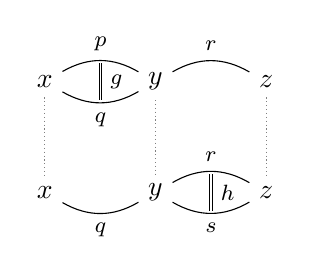
\begin{tikzpicture}[node distance=4em, baseline=(basenode.base)]
        \node[] (x1) {$x$};
        \node[right of=x1] (y1) {$y$};
        \node[right of=y1] (z1) {$z$};
        \node[below of=x1] (x2) {$x$};
        \node[right of=x2] (y2) {$y$};
        \node[right of=y2] (z2) {$z$};
        \draw[bend left] (x1) to node[above] (p) {\footnotesize$p$} (y1);
        \draw[bend right] (x1) to  node[below] (q1) {\footnotesize$q$} (y1);
        \draw[bend left] (y1) to node[above] (r1) {\footnotesize$r$} (z1);
        \draw[bend left] (y2) to node[above] (r2) {\footnotesize$r$} (z2);
        \draw[bend right] (y2) to  node[below] (s) {\footnotesize$s$} (z2);
        \draw[bend right] (x2) to node[below] (q2) {\footnotesize$q$} (y2);
        \draw[double, shorten >=.1em, shorten <=.1em] (p) to node[right] {\footnotesize$g$} (q1);
        \draw[double, shorten >=.1em, shorten <=.1em] (r2) to node[right] {\footnotesize$h$} (s);
        \draw[gray,densely dotted] (x1) to node (basenode){} (x2) (y1) to (y2) (z1) to (z2);
      \end{tikzpicture}%
      =%
      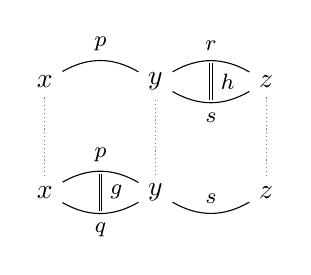
\begin{tikzpicture}[node distance=4em, baseline=(basenode.base)]
        \node[] (x1) {$x$};
        \node[right of=x1] (y1) {$y$};
        \node[right of=y1] (z1) {$z$};
        \node[below of=x1] (x2) {$x$};
        \node[right of=x2] (y2) {$y$};
        \node[right of=y2] (z2) {$z$};
        \draw[bend left] (x2) to node[above] (p) {\footnotesize$p$} (y2);
        \draw[bend right] (x2) to  node[below] (q1) {\footnotesize$q$} (y2);
        \draw[bend right] (y2) to node[above] (r1) {\footnotesize$s$} (z2);
        \draw[bend left] (y1) to node[above] (r2) {\footnotesize$r$} (z1);
        \draw[bend right] (y1) to  node[below] (s) {\footnotesize$s$} (z1);
        \draw[bend left] (x1) to node[above] (p2) {\footnotesize$p$} (y1);
        \draw[double, shorten >=.1em, shorten <=.1em] (p) to node[right] {\footnotesize$g$} (q1);
        \draw[double, shorten >=.1em, shorten <=.1em] (r2) to node[right] {\footnotesize$h$} (s);
        \draw[gray,densely dotted] (x1) to node (basenode){} (x2) (y1) to (y2) (z1) to (z2);
      \end{tikzpicture}%
    \end{sidecaption}
  \end{figure}%
  %
  One prove such a result by induction on $h$. Indeed, when
  $h\jdeq \refl r$, then both sides of the equation reduces through
  path algebra to $\ap {r\cdot\blank} (g)$. Now we are interested in
  this result when $x,y,z$ are all equal to $a$ by definition, and $p,q,r,s$
  are all equal to $\refl a$ by definition. In that case, one has that
  $\ap {\refl a\cdot \blank}$ and $\ap {\blank\cdot\refl a}$ both act
  trivially, and the equation becomes: $h\cdot g = g \cdot h$.

  One still has to prove that the function $\loopspace$ is an inverse
  for $\BB$. Given an abelian group $G$, the proof
  of~\cref{lemma:universal-cover-simply-connected} gives an
  equivalence between $\B\loopspace {(\BB G)}$ and the connected
  component of $\refl {\BG_\div}$ in $\BG_\div\eqto \BG_\div$. By
  definition, this is the classifying type of $\grpcenter(G)$. Being
  abelian, $G$ is isomorphic to its center
  (\cref{def:abelian-groups}), and so it yields an element of
  $\loopspace {(\BB G)} \eqto_{\typegroup} G$. %
  \marginnote[-1.5\baselineskip]{%
    If $X \ptdweto Y$ denote the type of pointed equivalences between
    pointed types $X,Y:\UUp$, then the univalence axiom implies that
    there is an equivalence
    \begin{displaymath}
      (X=Y) \weq (X \ptdweto Y).
    \end{displaymath}%
  }%
  Conversely, take a pointed simply connected $2$-type $(A,a)$. We
  want to produce a pointed equivalence
  $\Phi : (A,a) \equivto \BB (\loopspace {(A,a)}) $. One should first
  notice that the function
  \begin{fullwidth}
    \begin{equation}
      \label{eq:loopspace-A-abelian}%
      \ev^a_{refl a}{\B\loopspace \left( \BB (\loopspace {(A,a)}) \right)}
      \jdeq \conncomp{((a\eqto a)\eqto (a\eqto a))}{\refl{a\eqto a}} \to (a\eqto a,\refl a).
    \end{equation}
  \end{fullwidth}
  that maps a path
  \begin{displaymath}
    (p,!):(a\eqto a,\settrunc{\refl{a\eqto a}})\eqto (a\eqto a,\settrunc{\refl{a\eqto a}})
  \end{displaymath}
  to the evaluation $p(\refl a): a\eqto a$ is an equivalence, because
  $\loopspace (A,a)$ is an abelian group.

  %% OLD MATERIAL, can still be useful.
  %%
  % We will now provide
  % \begin{displaymath}
  %   \Phi : \BB {(\loopspace {(A,a)})} \ptdto (A,a)
  % \end{displaymath}
  % such that $\loopspace(\Phi)$ is the previous equivalence.
  % To be able to
  % express $\Phi$, we need a small gadget about truncations of
  % function
  % types: for types $X,Y:\UU$, given an element
  % $f_0:\setTrunc{X\to Y}$, one constructs a map
  % $\lceil f_0 \rceil : \setTrunc X \to \setTrunc Y$; the type of
  % $\lceil f_0 \rceil$ being a set, one might as well suppose that
  % $f_0 \jdeq \settrunc f$ for some $f:X\to Y$; then we set
  % $\lceil f_0 \rceil (\settrunc x) = \settrunc{f(x)}$, which
  % suffices
  % in order to define $\lceil f_0 \rceil$ entirely because its
  % codomain
  % $\setTrunc Y$ is a set. If we assume the axiom of
  % choice\footnote{What is the status of AC in this book??}, then
  % $\lceil \blank \rceil$ is injective when $Y$ is a set.
  %%
  We will now define a pointed map
  $\Phi : (A,a) \ptdto \BB (\loopspace {(A,a)})$, and prove
  subsequently that this is an equivalence. Let $T : A \to \UU$ be the
  type family (of sets) define by
  \begin{displaymath}
    T(a') \defequi \sum_{\alpha:\setTrunc{(a\eqto a)\weq(a\eqto a')}}
    \prod_{p:a\eqto a'}\alpha=\settrunc {p\cdot\blank}
  \end{displaymath}
  We claim that $T(a')$ is contractible for all $a':A$. By
  connectedness of $A$, it is equivalent to show that $T(a)$ is
  contractible. However,
  \begin{align*}
    T(a)
    &\jdeq \sum_{\alpha:\setTrunc{(a\eqto a)\equivto(a\eqto a)}}\prod_{p:a\eqto a}
      \alpha = \settrunc {p\cdot \blank}
    \\
    &\weq \sum_{\alpha:\setTrunc{(a\eqto a)\equivto(a\eqto a)}} \alpha = \settrunc{\id_{a=a}}
    \\
    &\weq 1
  \end{align*}
  Then, we define $\Phi (a')$ to be the element
  $(a\eqto a', \kappa_{a'}):\univcover \UU {a\eqto a}$ where
  $\kappa_{a'}$ is the first projection of the center of contraction
  of $T(a')$. In particular, following the chain of equivalences
  above, $\Phi(a)$ is defined as
  $(a\eqto a, \settrunc{\refl {a\eqto a}})$, hence $\Phi(a)$ is
  trivially pointed by a reflexivity path. To verify that $\Phi$, thus
  defined, is an equivalence, one can use connectedness of
  $\BB(\loopspace (A,a))$ and only check that
  $\inv\Phi(a\eqto a,\settrunc{\refl {a\eqto a}})$ is
  contractible. However, there is a canonical equivalence of type:
  \begin{displaymath}
    \inv\Phi(a\eqto a,\settrunc{\refl {a\eqto a}}) \equivto \sum_{a':A}
    \sum_{\varphi : (a\eqto a) \equiv (a\eqto a')}\settrunc{\varphi} = \kappa_{a'}.
  \end{displaymath}
  So we will show that the type on the right hand-side is
  contractible. For an element $a':A$ together with
  $\varphi: (a\eqto a) \equiv (a\eqto a')$ such that the proposition
  $\settrunc \varphi = \kappa_{a'}$ holds, a path between
  $(a,\id_{a\eqto a},!)$ and $(a',\varphi,!)$ consists of a path
  $p:a\eqto a'$ and a path $q:(x\mapsto p x) \eqto \varphi$. We have a
  good candidate for $p$, namely $p\defequi \varphi(\refl
  a):a\eqto a'$. However we don't have quite $q$ yet. Consider, for any
  $a':A$, the function
  \begin{displaymath}
    \ev_{\refl a}^{a'} :
    \left(
      (a\eqto a, \settrunc{\refl{a\eqto a}} ) =
      (a\eqto a', \kappa_{a'} )
    \right)
    \to (a\eqto a')
  \end{displaymath}
  defined as $(\psi,!) \mapsto \psi(\refl a)$.  Note that
  $\ev_{\refl a}^{a}$ is precisely the equivalence
  $\B\loopspace{(\BB\loopspace(A,a))}_\div \equiv (a=a)$ described
  in~\cref{eq:loopspace-A-abelian}. Hence, by connectedness of $A$,
  one gets that the proposition $\isEq(\ev_{\refl a}^{a'})$ holds for
  all $a':A$. In particular, because the propositions
  $\settrunc \varphi = \kappa_{a'}$ and
  $\settrunc {p\cdot\blank} = \kappa_{a'}$ holds, one gets elements
  $(\varphi,!)$ and $(x\mapsto px,!)$ in the domain of
  $\ev_{\refl a}^{a'}$. Their images $\ev_{\refl a}^{a'}(\varphi,!)$
  and $\ev_{\refl a}^{a'}(x\mapsto px,!)$ are both identifiable with
  $p$. By composition, we obtain a path
  $(x\mapsto px,!)\eqto (\varphi,!)$ in the domain. The first
  component provide the path $q:(x\mapsto px) \eqto \varphi$ that we
  wanted.
\end{proof}

\subsection{Higher deloopings}

The function $\BB$ defined in the proof
of~\cref{thm:abelian-groups-weq-sc2types} provides a delooping of
$\BG$ whenever $G$ is abelian. That is, there is an identification
$\loops \BB G \eqto \BG$. A systematic way of obtaining such
deloopings has been developed by David W\"{a}rn\footcite{Warn-EM},
that can be applied here to give an alternative definition of $\BB G$,
and to obtain further deloopings of it.

\begin{definition}[W\"{a}rn]
  Given a pointed type $X$, the type of {\em $X$-torsors} is
  \begin{displaymath}
    TX \defequi \sum_{Y : \UU} \Trunc{Y} \times \left( \prod_{y:Y}(Y,y) \ptdweto X \right).
  \end{displaymath}
  The type of {\em pointed $X$-torsors} is
  $TX_\ast \defequi \sum_{t : TX}\fst t$.
\end{definition}
The usefulness of these definitions in the context of deloopings comes
from the following proposition.
\begin{lemma}[W\"{a}rn]
  Let $X$ be a pointed type. If $TX_\ast$ is contractible, then for
  any pointed $X$-torsors $(t,y)$, the pointed type $(TX,t)$ is a
  delooping of $X$.
\end{lemma}
\begin{proof}
  Suppose $(t,y)$ is a center of contraction for $TX_\ast$. By
  contracting away (\cref{lem:contract-away}) in two different ways,
  we obtained a composition of equivalences:
  \begin{displaymath}
    (t \eqto t) \equivto \sum_{u : TX}\fst u \times (t \eqto u) \equivto \fst t 
  \end{displaymath}
  that maps $\refl t$ to $y$. In other words, this equivalence,
  trivially pointed, presents $(TX, t)$ as a delooping of
  $(\fst t, y)$. Moreover, the $X$-torsor $t$ comes by definition with
  an identification $(\fst t,y) \ptdweto X$. So in the end, we have an
  equivalence $(TX, t) \ptdweto X$.
\end{proof}

\begin{exercise}\label{xca:sections-as-dependent-functions}
  Recall that a {\em section} (see~\cref{def:surjection} and its
  accompanying footnote) of a function $f:A \to B$ is a function
  $s: B \to A$ together with an identification $f\circ s \eqto \id_B$.
  Construct an equivalence from the type $\secfun f$ of sections of
  $f$ to the type $\prod_{b:B}\sum_{a:A}b \eqto f(a)$.
\end{exercise}

Consider the evaluation function
$\ev_{X_\div,Y} : (X_\div \eqto Y) \to Y$ (defined by path-induction,
sending $\refl X$ to the distinguished point of $X$). In other words,
the function $\ev_{X_\div,Y}$ takes an identification of $X_\div$ with
$Y$ and returns the point in $Y$ corresponding to the distinguished
point of $X$ under this identification.  Applying
\cref{xca:sections-as-dependent-functions} to $\ev_{X_\div,Y}$ we get
an equivalence of type
\begin{displaymath}
  TX \equivto \sum_{Y : \UU} \Trunc{Y} \times \secfun(\ev_{X_\div,Y}).
\end{displaymath}
This alternative description of the type of $X$-torsors is the key
ingredient to compare W\"arn's delooping of the classifying type of
an abelian group with our.

\begin{lemma}\label{lem:warn-abelian-group}
  For any abelian group $G$, the type $T(\BG)$ can be identified with
  $\BB G$.
\end{lemma}
\begin{proof}
  Let $G$ be an abelian group. We first construct, for each type
  $Y$, a function
  $f_Y : \Trunc{Y} \times \secfun(\ev_{\BG_\div,Y}) \to
  \setTrunc{\BG_\div \eqto Y}$, and then prove that $f_Y$ is an
  equivalence. Given a type $Y$ and an element
  $(!,s) : \Trunc{Y} \times \secfun(\ev_{X_\div,Y})$, we can easily
  prove that $Y$ is connected: being connected is a proposition, so
  we can assume that we have an actual $y:Y$ and then
  $s(y) : \BG_\div \eqto Y$ proves that $Y$ is as connected as
  $\BG_\div$ is. Consequently $s$ must send $Y$ into one of the
  connected component of $\BG_\div \eqto Y$, that we choose to be
  $f_Y(!,s)$. With this definition, the fiber of $f_Y$ at any given
  $c : \setTrunc{\BG_\div \eqto Y}$ can be identified with the type
  of sections $s$ of $\ev_{\BG_\div,Y}$ with values in $c$. However,
  for any $Z$ and $p: \BG_\div \eqto Z$ the restriction of the
  evaluation
  $\ev_{\BG_\div,Z}\restriction_p : \conncomp{(\BG_\div \eqto Z)} p
  \to Z$ is an equivalence: indeed, by induction, we only have to
  show it for $p\jdeq \refl {\BG_\div}$, in which case
  $\ev_{\BG_\div,\BG_\div}\restriction_{\refl {\BG_\div}}$ is
  exactly the map $\B\grpcenterinc G$ defined in
  \cref{sec:center-group}, which is an equivalence since $G$ is
  abelian by \cref{def:abelian-groups}. Thus, given any $p$, the
  fiber of $f_Y$ at $\settrunc p$ is contractible. Being
  contractible is a proposition, hence a set, so it follows that the
  fiber of $f_Y$ at any $c:\setTrunc{\BG_\div \eqto Y}$ is
  contractible. In other words, $f_Y$ is an equivalence, as
  announced. We have thus a chain of equivalences:\footnote{Notice
    that the construction of an equivalence
    $TX \equivto \univcover \UU {X_\div}$ that we carried for
    $X\jdeq\BG$ relies only on $X_\div$ being connected and
    $\ev_{X_\div,X_\div}\restriction_{\refl {X_\div}}$ being an
    equivalence. Such types $X$ are called \emph{central} and are
    studied in details by~\citeauthor{BCFR}\footnotemark{}.}.%
  \footcitetext{BCFR}
  \begin{displaymath}
    T(\BG) \equivto \sum_{Y : \UU} \Trunc{Y} \times \secfun(\ev_{X_\div,Y})
    \equivto \sum_{Y : \UU} \setTrunc{\BG_\div \eqto Y} \jdeq \BB G
  \end{displaymath}
\end{proof}

Notice that where W\"arn's method shines, compared to our, is in
producing further delooping $\B^n G$ for $n\geq 3$.

\section{Stabilization}

%%% Local Variables:
%%% mode: LaTeX
%%% fill-column: 144
%%% latex-block-names: ("lemma" "theorem" "remark" "definition" "corollary" "fact" "properties" "conjecture" "proof" "question" "proposition" "exercise")
%%% TeX-master: "book"
%%% TeX-command-extra-options: "-fmt=macros"
%%% compile-command: "make book.pdf"
%%% End:
